% ComplexNetworks_McGarry.tex
% Submitted to: Journal of Computers in Biology and Medicine 
% https://www.journals.elsevier.com/computers-in-biology-and-medicine/
% started:       4/1/18
% completed: 17/2/18
% reviewers: 2/3/18
% completed 

\documentclass[a4paper,8pt,twocolumn,5p]{elsarticle}
\usepackage{amssymb}
\usepackage{amsmath}
\usepackage{epsf}
\usepackage{graphicx}
\usepackage{epstopdf}
\usepackage{natbib} 
\usepackage{mathtools}
%\usepackage[margin=1in]{geometry}
\usepackage{array}% http://ctan.org/pkg/array
\usepackage{amsmath} 
\usepackage{algorithmicx}
\usepackage{algorithm}
\usepackage{algpseudocode}
%\usepackage{subfigure}
\usepackage{subcaption}
\usepackage{verbatim}
\usepackage{mwe}
\usepackage{tikz}
\usetikzlibrary{matrix,fit}

\begin{document}
\begin{frontmatter}
\title{Complex network theory for the identification and \\assessment of candidate protein targets}
%\author{Ken McGarry and Sharon McDonald}
%\author[label2,label3]{Author2}
%\address{School of Pharmacy and Pharmaceutical Sciences, \\University of Sunderland, City Campus, \\Sunderland, SR1 3SD, UK}

\author[add1]{Ken McGarry}
\ead{ken.mcgarry@sunderland.ac.uk}
\author[add2,add3]{Sharon McDonald}
%\ead{sharon.mcdonald@sunderland.ac.uk}
\address[add1]{Faculty of Health Sciences and Well-being, \\University of Sunderland, City Campus, \\Sunderland, SR1 3SD, UK}
\address[add2]{Faculty of Computer Science, \\University of Sunderland, St Peters Campus, \\Sunderland, SR6 ODD, UK}

\begin{abstract}
In this work we use complex network theory to provide a statistical model of the connectivity patterns of human proteins and their interaction partners. Our intention is to identify important proteins that may be predisposed to be potential candidates as drug targets for therapeutic interventions. Target proteins usually have more interaction partners than non-target proteins, but there are no hard and fast rules for defining the actual number of interactions. We devise a statistical measure for identifying hub proteins, we score our target proteins with gene ontology annotations, the important drugable protein targets are likely to have similar biological functions that can be assessed for their potential therapeutic value. Our system provides a statistical analysis of the local and distant neighborhood protein interactions, of the discovered proteins, using complex network measures. This approach builds a more accurate model of drug-to-target activity and therefore, the likely impact on treating diseases. We integrate high quality protein-interaction data from the HINT database, disease associated proteins from the DrugTarget database, biological knowledge from Gene Ontology and further drug information from DrugBank. RandomForest classifier models are built on this information which are used to identify previously unclassified proteins, we validate and corroborate these findings from the available literature.
\end{abstract}
\begin{keyword}
Complex network theory \sep link-clustering \sep protein interactions \sep ontologies 
\end{keyword}
\end{frontmatter}

\section{Introduction}
A major factor in understanding the effects of diseases and their inter-relationships, is to appreciate the role and functionality of protein interactions. Protein interactions are key to the majority of functions occurring in the cell and also account for several signaling mechanisms for processes external to the cell \cite{Nabieva05}. The connectivity of interacting proteins (interactome) when mapped as a net-work reveals a complex web of relationships. Some proteins have many connections while others are sparsely connected. The application of computational techniques, such as clustering, can also reveal the modular nature of proteins as they cooperate in various activities \cite{McGarry2013}. Researchers have modified graph theoretic methods to tackle the issues inherent with protein interaction networks, or have implemented predicative algorithms for identifying protein function \cite{McGarry07a}. The identification of  interesting sub-graphs, using a combination of clustering and classification methods, has been the focus of increased interest. These computational techniques are essential to unraveling the complex nature of genes, proteins and their relationship with diseases.

 A high degree of heterogeneity exits in the relationship between genes and disorders: some diseases are implicated with a small number of genes, while some medical problems, such as colon cancer and deafness, have been associated
with more than thirty genes \cite{Menche2015}. However, most genes are generally associated with only a few diseases, although there are notable exceptions. For example, genes such as the tumor suppressor gene TP53 is known to be implicated with up to ten disorders. Clearly, these hub genes play an important role as causal factors for disease. Further, diseases that appear to be interlinked with the hub genes and can cause multiple problems when the implicated genes become defective \cite{Ghiassian2015}. The human disease network as it is now called is providing a new way of thinking regarding how diseases occur  \cite{Barrenas2009}. The objective is to develop novel drug products and to potentially reposition existing drugs to new targets  \cite{Yue2017}.  However, it does beg the question, how many potential protein targets are there? \cite{Overington2006}. Some may be completely undruggable, while others can only be perturbed by targeting their network neighborhood proteins. Currently, full knowledge of the proteome and interaction targets is many years away from completion  \cite{Barabasi2011}.

%%%%%%%%%%%%%%%%% Figure %%%%%%%%%%%%%%%%%
\begin{figure*}[ht]
%\epsfysize=4.0cm \leavevmode
  \begin{center}
 \includegraphics[width=17cm,height=12cm]{/Latex/DiseaseNets/targets2hubs.jpg} % OK
  \end{center}
\special{center} \caption{Small fraction of the protein network with drug targets colored yellow and slightly larger in size, non-targets are colored light blue. However, based on their connectivity patterns, their biological and complex network statistics, some of the non-targets may be prove to be viable drug targets.}
\label{small_net}
\end{figure*}
%%%%%%%%%%%%%%%%%%%%%%%%%%%%%%%%%%%%

Recent studies based on the modelling of cooperating modular groups of genes have suggested that diseases themselves are in fact network like \cite{BauerM2011}. The concept of the human disease network or \emph{diseasome} is now considered a useful means of developing new drug products to tackle and combat diseases \cite{He2011}.  Figure \ref{small_net} shows an overview of the drugable target proteins.  Gene essentiality has been considered \cite{Rancati2018}. The drug-target network alluded to by Yildirium {\it et al}, is based on similar concepts to the diseaseome by differentiating protein targets into essential, disease or target types \cite{Yildirium2007}. Based on these criteria they were able to deduce that rational drug design over the last 10 years results in more specific targeting of proteins

For other diseases  the issue, however, is not so straight-forward.  Within a given cluster, a number of genes may compensate for the malfunction of one gene: consequently making the identification of the faulty gene more difficult \cite{LeePark2008}.  However, recent work has identified an underlying set of organizing principles that can be used to assess and identify the structures involved, we  discuss these criteria in section two. A good overview of the technologies and challenges such as the cellular organization and the detection of structural motifs involved in network-based approaches to understanding diseases can be found in Barabasi  \cite{Barabasi2004}.  We can improve our knowledge and understanding of the mechanisms of disease based on a better understanding of protein targets and non-targets and may suggest alternative therapeutic interventions \cite{McGarry2017a,McGarry2017b}. 

\subsection{Related work}
Similar systems to ours have been developed such as the system developed by Yu et al, which considers the problem as one of module distance estimation with the understanding that the human interactome is still incomplete and with all the uncertainty inherent \cite{Yu2016}. Yu's ultimate goal was concerned with repositioning drugs for different diseases. The modules are composed of drug-protein pairs and all are involved with cancer specific functions, the disease module distance metric was able to identify several candidate drugs. The MBiRW method developed by Luo et al. (2016), uses a bi-random walk to measure similarity of drugs and diseases \cite{Luo2016}. MBiRW uses novel similarity measures and is well validated against gold standard data but lacks target information and biologically relevant information.  The CommWalker algorithm devised by Luecken uses a random walk approach to sample the proteins assigned to functional modules \cite{Luecken2017}. For robustness, the modules are formed by three different link-analysis procedures and an average walk will produce a goodness of fit value. The walks are terminated when they have approach a critical value. At each step the functional GO annotation is averaged out to calculate  the module homogeneity, scores are then combined to enable each module to be ranked on its biological plausibility. 
 
The closest work to ours tackles the challenges and opportunities of integrating biological knowledge in the form of annotations from gene ontology (GO). For example, Hsing {\it et al} used GO to build classifiers to identify hub proteins, these are highly connected proteins with many interaction partners \cite{Hsing2008}. However,  the classifiers performed badly on some proteins through lack of suitable annotations. Work by Zhang {\it et al} explored the issues of identifying protein interaction partners through use of GO terms \cite{SBZhang2016}. Support Vector Machine classifiers were constructed on the GO annotated PPI data and good accuracy was achieved on predicting the likely interaction partners. Research by Fu {\it et al} explored the likelihood that  intrinsic disorder proteins will form highly interconnected hubs  and potentially drug targets \cite{Fu2015}. Again, the usefulness of GO was employed to annotate and analyze the relationships. 

We extend all this previous work by adding novel analysis of the hub and target proteins using complex network theory and community structure of the protein interactions. Furthermore, we annotate the protein interactions with GO terms to help identify novel protein targets. Thus we are able to generate target protein candidates for use by other researchers to conduct biological experiments in the lab. The remainder of this is paper is structured as follows: section two discusses the methods including the architecture of our system and the sources of data and knowledge, section three describes the experimental  results, section four presents the discussion and finally section five presents the conclusions and future work. 


\section{Materials and methods}
\subsection{Data and knowledge sources}
The candidate drugs have known on-target and off-target proteins, this knowledge is augmented by accessing protein-to-protein interactions found in the HINT database \cite{Das2012}. This database contains high-quality protein-protein interactions from 8 interactome resources (BioGRID, MINT, iRefWeb, DIP, IntAct, HPRD, MIPS and the PDB). The database contains 12,429 unique proteins with 59,128 interactions between them. http://hint.yulab.org/. This data was further augmented by high quality protein interactions from the BioPlex database maintained by Harvard Medical School (http://bioplex.hms.harvard.edu/) \cite{Huttlin2015}.

Drug and protein target data was obtained from DrugCentral, this is a comprehensive drug information resource for FDA drugs and drugs approved outside USA. The resources can be searched using: drug, target, disease, and pharmacological action. The information resource is created and maintained by the Division of Translational Informatics at University of New Mexico. (as of 8th January 2018, http://drugcentral.org/). The data is particularly suited for our purposes, because we use the drugname, protein targets and protein type \cite{Ursu2017}.

Gene ontology (GO) provides useful biological information and it is recognized as the {\it de facto} standard for gene product annotation \cite{Ashburner00}. This enables an assessment to be made regarding the biological plausibility of the interacting proteins to observe the extent they actually cooperate in viable biological functions rather than random or spurious associations. The GO terms are organized to represent the three main aspects of biology: molecular functions (MF), cellular components (CC) and biological process (BP). For each protein, enrichment was performed using the GO-slim version of the gene ontology (GO), the enrichment is based on similarity measures using information content techniques \cite{Davis2010}. We mapped our low-level annotations to several high-level GO-slim terms, in the generic version we used, 149 terms are available.

Any proteins without GO terms are removed and  all remaining proteins are annotated the GO-slim version  (http://www.geneontology.org/page/go-slim-and-subset-guide) simplifies the terms. GO-slims are subsets of terms in the ontology that give a broad overview of the ontology content.  GO-slims do this without including the detail of the specific fine grained terms and therefore simplify computational model building, we discover that accuracy is not greatly compromised \cite{Davis2010}. We obtain accuracy's that are comparable to other work that uses the full GO terms.

The GO-slim annotated proteins are used to build a RandomForest classifier \cite{Breiman2001}.  Random Forests are a supervised ensemble classification technique requiring class labels, where a group of weak models combine to form a powerful model. Several decision trees are created (hence a forest) with random sampling used as the attribute to split on, there is a direct correlation between the number of trees in the forest and the accuracy. Another important advantage of the Random Forest classifier is that the predictor variables are ranked according to importance using the Gini impurity measure and is used for the calculation of splits during training. 

The RandomForest was assessed using standard classifier metrics:\\

\noindent Accuracy = (TP + TN) / (TP+ TN + FP + FN)\\
Sensitivity = TP / (TP + FN) \\
Specificity = TN / (TN + FP) \\
PPV = TP / (TP + FP) \\
NPN = TN / (TN + FN) \\

\noindent Where: TP is a True Positive; TN is a True Negative; FP is a False Positive and FN is a False Negative. PPV is the Positive Predictive Value and the NPV is the Negative Predictive Value. ROC and PR curves were plotted using these values.

\subsection{Software implementation and availability}
The system was implemented using the R language with the RStudio programming environment, on an Intel Xenon CPU, 64-bit with dual processors (3.2GHz) and 128 GB of RAM. The igraph  package by Kolaczyk was the main software used \cite{Kolaczyk2014}. Other general purpose packages for data manipulation, transformations and plotting include; ggplot2, dplyr and ontologySimilarity.  The RandomForest package by Liaw allowed the building and testing of the classifier models \cite{Liaw2002}. Our R code and data files that generate the tables, diagrams and functional code described in this paper are freely available on GitHub for download: \\https://github.com/kenmcgarry/ComplexNetworks

\subsection{Complex network theory}
Graph theoretic methods are suitable to any application where the entities of interest are linked together through various associations or relationships.  Quite diverse application areas such as social network analysis and biological networks are particularly suited to the mathematics of graph construction, traversal and inferencing. A graph G = (V, E) consists of a set of nodes often called vertices V and a set of links called edges E. The links in this case are undirected, that is to say there is no implied direction to the relationship in the sense that A causes B.

The criteria we use to determine the relevance of disease connectivity is based upon recent discoveries,   it is likely that the essential genes and the disease genes encode the hubs \cite{Vidal2011} and that gene network topology is unlikely to encode the information to deduce disease modules \cite{Ghiassian2015}. In algorithm \ref{alg1}, we detail our computational  methods of discovering the disease modules.

Closeness centrality (CC) of protein i is the sum of graph-theoretic distances from all other proteins in the network, where the distance $d(v_i, v_j)$ from one protein $i$ to another $j$ is defined as the number of links in the shortest path from one to the other, where N is the number of all proteins in the network. The closeness centrality of protein $i$ in a network is given by the equation:

\begin{equation}\label{closeness}
     CC(v_i) =  \frac{N - 1}{\sum_{j} d(v_i,v_j)}
\end{equation}


Betweenness centrality assesses the extent of influence a protein has in facilitating communication between pairs of proteins and is defined as the fraction of shortest paths going through a given node \cite{Freeman1979}. In the PPI network, then the CB of a node $v$ is given by: 

\begin{equation}\label{betweenness}
     CB (v) =  \sum_{s \not= t \not= \nu \in V} \frac{\sigma (s,t, | v)}{\sigma (s,t)}
\end{equation}

Where: $\sigma (s, t, | v)$ is the total number of distinct shortest paths from node $s$ to node $t$ passing through $v$, $\sigma (s,t)$ is the total number of shortest paths between node $s$ and node $t$  irrespective of whether they pass through node $v$ or not. 

Since complex networks (graph theory) can be very large, real-world applications may consist of thousands of nodes and tens of thousands of connections, there is often a need to query if two particular nodes are connected and if so how distance are they are. Detection and assessment of  the {\it shortest path} is important to centrality measures and can be defined as when two nodes $i$ and $j$ are connected if there exists  a sequence of connections that  connect $i$ and $j$. The length of a path is the number of connections between them, denoted by $d_{ij}$. In biology, two proteins may not interact directly but may communicate through a signaling cascade of other proteins. Small path lengths from tightly coupled networks tend to give high clustering coefficients as derived by equation \ref{clustercoeff}, random networks have low clustering coefficients compared with real-world networks. 

\begin{equation}\label{clustercoeff} 
     C_{i}  =  \frac{2\mid\{e_{jk} \}\mid}{k_{i}(k_{i} - 1)} : v_{j}, v_{k} \in N_{i}, e_{ij} \in E
\end{equation}

Where $V = v1, v2  ... vn$ are a set of $n$ vertices and $E$ a set of edges, where $e_{ij}$ denotes an edge between
vertices $v_i$ and $v_j$ $k_i$ refers to the vertex neighbours. The neighbourhood $N$, for a vertex $v_i$, is its immediately connected neighbors as follows:

\begin{equation}\label{neighbour}
     N_{i}  =  \{v_{j}\}:e_{ij} \in E
\end{equation}

The degree $k_i$ of a vertex is the number of vertices in its neighborhood $| Ni |$.  Making the clustering coefficient $C_i$ for a vertex $v_i$ the proportion of links between the vertices within its neighborhood divided by the number of links that could possibly exist between them. In addition undirected graphs have the property that $e_{ij}$ and $e_{ji}$ are considered identical. Therefore, if a vertex $v_i$ has $k_i$ neighbor, only the following edges could exist among the vertices within the neighborhood. 

The clustering coefficient is used to estimate the density of the immediate neighborhood of each vertex  and formally, for undirected graph $G = (V;E)$, define the neighbor set of $v_i \in V$, denoted by $N_{v_i}$ .  A high cluster coefficient indicates a high level of interconnection between members of a node's neighboring nodes. These measures return a value of one if every neighbor connected to $v_i$ is also connected to every other vertex within the neighborhood $n$, and zero if no vertex that is connected to $v_i$ connects to any other vertex that is connected to $v_i$.  The clustering coefficient for the entire network is the average of the clustering coefficient for each vertex:

\begin{equation}\label{watts}
    C = \frac{1}{n} \sum_{i=1}^n C_{i}
\end{equation}

We therefore expect that hub proteins on average have a higher clustering coefficients than non-hubs. This was confirmed by our experimental work but the important proteins are not identified by connectivity numbers alone, the location of a key protein is also by its position (topology) in the network.

\begin{algorithm}
\caption{\\Build Random Forest classifier and complex network}\label{alg1}
\begin{algorithmic}[1]
\scriptsize
\Procedure{Build RF Classifier}{$HINT,DrugTarget, GO-slim$}
   \State{\textit{\bf do initialize}}
       \State \hspace{\algorithmicindent} protein list $\gets \mbox {annotate with target/nontarget labels}$
       \State \hspace{\algorithmicindent} protein list $\gets \mbox {annotate with GO-Slim}$
       \State \hspace{\algorithmicindent} Remove proteins with $<$ 1 GO-Slim annotation
       \State \hspace{\algorithmicindent} proteins list $\gets \mbox {randomly select 1,443 nontargets}$
       \State \hspace{\algorithmicindent} proteins list $\gets \mbox {80/20 split between train and test}$
       \State \hspace{\algorithmicindent} unseen list $\gets \mbox {randomly select samples with unknown labels}$
       \State \hspace{\algorithmicindent} proteins matrix $\gets \mbox {convert list to binary matrix}$
   \State{\textit{\bf end initialize}}  \\ \\

    \hspace{\algorithmicindent} PPInetwork $\gets \mbox {igraph builds complex network }$\\
    \hspace{\algorithmicindent} NetStatistics $\gets \mbox {calculate k-coreness for all nodes }$\\
 
   \While{\State\text{accuracy$ \leq $accuracy from last iteration}}
          \State\hspace{\algorithmicindent} RF parameters$\gets \mbox {(Num Trees, Cutoff )}$
          \State\hspace{\algorithmicindent} RF accuracy$\gets \mbox {test data }$
          \State\hspace{\algorithmicindent} Candidate list$\gets \mbox {RFmodel(unseen data)}$
   \EndWhile      \\
   
   
       \State \textbf{return} $PPInetwork, NetStatistics, RandomForest$
\EndProcedure
\normalsize
\end{algorithmic}
\end{algorithm}

Referring to algorithm \ref{alg1}, lines 2-9 perform the initialization of key values. Based on the available information on protein targets we label proteins as either a target or nontarget. All proteins are then annotated with GO-slim, any protein without an annotation of some form is removed from the study. Since we are left with 1,443 targets, we randomly select the same number from our list of nontargets. A binary matrix for training the random forest is made which is then split 80/20 for train/test data, the matrix consists of a series of 1's' for presence of a GO-slim term and 0's if it is not for each protein with the class label for target/nontarget identify.

Lines 12 and 13 build the protein to protein interaction network (PPI) and calculate a number of statistics, the most important is the k-coreness for each protein. Lines 15-20 handle the training of the Random Forest classifier, we modify the number of tree's, the cutoff (the ‘winning’ class for an observation is the one with the maximum ratio of proportion of votes to cutoff) to obtain the best model. Line 18 involves passing the unseen data through the trained RF classifier and generates a list of candidate targets. 

A graph is k-connected if every pair of vertices is connected through at least k distinct paths, that do not share edges. This property is related to the strength of a network, a k-connected network remains connected whenever fewer than k links are removed or broken. The k-core of graph is a maximal subgraph in which each vertex has at least degree k. The coreness of a vertex is k if it belongs to the k-core but not to the (k+1) core. The cores represent an important subgraph that contain functions of biological significance. The emergence of hubs is a consequence of the scale-free property of networks. Hubs can be found in many real networks and have a significant impact on the topology, but they cannot be observed in a random network.


\section{Results}
The first stage was to assess the impact of study bias of the known protein connectivity patterns. The data are the result of scientific experiments that may have concentrated on the better known or more  'glamorous' proteins. That is to say proteins with few connections may be the result of neglect on the part of the scientific community and not because these proteins do not have an important role.

In figure \ref{barplot1} the frequency counts of the types of protein targets is displayed, the most predominant type is GPCR. We removed any protein type with fewer than 50 records as they were deemed unlikely to produce successful classifiers.  

%%%%%%%%%%%%%%%%% Figure %%%%%%%%%%%%%%%%%
\begin{figure}[h]
\centering
 \includegraphics[width=8cm,height=7cm]{/Latex/DiseaseNets/barplot1.PDF} % OK
\centering \caption{Breakdown of protein types (13,735 unique proteins) from DrugCentral database. }
\label{barplot1}
\end{figure}
%%%%%%%%%%%%%%%%%%%%%%%%%%%%%%%%%%%%

We created the protein networks using the available proteins. In figure \ref{powerlaw} the degree of the network is plotted against the cumulative distribution function and it is evident that a powerlaw exists in the network. That is we have many proteins with few connections but there are a small number of proteins with several hundred connections.

%%%%%%%%%%%%%%%%%%%%%%%%%%%%%%%%%%%%
\begin{figure}[h]
\centering
\includegraphics[width=8cm,height=7cm]{/LaTex/DiseaseNets/degree.PDF} % second figure itself
\centering \caption{Protein network degree - power law is evident indicating the non-random network structure, the dotted line represents the 90th percentile cut-off point for determining if a protein is a hub. In this network, a degree of 17 is required giving 300 hubs.}
\label{powerlaw}
\end{figure}
%%%%%%%%%%%%%%%%%%%%%%%%%%%%%%%%%%%%

Complex networks were constructed using the protein interaction data and annotated each node with information regarding its status as a drug target, disease protein, hub protein, essential protein or function simply unknown. The overall network statistics based on connectivity patterns of 15726 nodes with 109,953 links gave: Modularity  of 0.37, Average path length of 3.81,  Transitivity  of 0.053, Diameter  of 11 and is fully connected with no disconnected (isolates) proteins. Table \ref{bet} shows the top 20 proteins ordered according to the {\it betweenness} statistics, this produces a very large value and is related to the {\it degree } of each individual node, these nodes have the largest number of connections to other proteins. The {\it  closeness} statistic is reasonably constant for these 20 proteins and implies that they have similar characteristics. The {\it hubness} value also varies little with these proteins and suggests that connectivity patterns are similar. The {\it centrality} measure is computed using the alpha centrality method, which is less likely to encounter problems with asymmetric matrices. The {\it community} measure indicates that these 20 proteins generally cooperate with few other communities or modules. A community is usually interpreted as a biological function or process. However, we must be careful not to infer too much from the network statistics alone the next stage is to annotate the network proteins with gene ontology (GO) terms. Determining biological plausibility through GO provides a more valid interpretation.

% latex table generated in R 3.4.0 by xtable 1.8-2 package
% Fri Jan 26 14:15:38 2018
\begin{table}[ht]
\centering \scriptsize \caption{Highest scoring 20 proteins ordered according to {\it betweenness}}
\label{bet}
\begin{tabular}{lllllll}
  \hline
 & close & degree & between & hub & central & comm \\ 
  \hline
HSP90AB1 & 5e-08 & 454 & 1353987 & 0.093 & 15 & 13.0 \\ 
  GRB2 & 6e-08 & 452 & 1228333 & 0.12 & 18 & 18.0 \\ 
  GOLGA2 & 5e-08 & 340 & 632816 & 0.13 & 36 & 8.0 \\ 
  ATXN1 & 4e-08 & 276 & 593291 & 0.051 &  29 & 11.0 \\ 
  ZDHHC17 & 3e-08 & 249 & 502844 & 0.053 &  33 & 11.0 \\ 
  KDM1A & 3e-08 & 224 & 399557 & 0.069 & 32 & 11.0 \\ 
  TRIM27 & 4e-08 & 258 & 393388 & 0.12 & 65 & 8.0 \\ 
  KRT40 & 3e-08 & 333 & 379048 & 0.14 & 58 & 8.0 \\ 
  MAPK6 & 3e-08 & 201 & 363744 & 0.058 &  47 & 11.0 \\ 
  UBE2I & 4e-08 & 202 & 351061 & 0.063 &  58 & 11.0 \\ 
  HSPA8 & 3e-08 & 199 & 347256 & 0.038 & 37 & 11.0 \\ 
  EGFR & 4e-08 & 196 & 339368 & 0.05 &  24 & 11.0 \\ 
  LZTS2 & 4e-08 & 244 & 338341 & 0.094 &  12 & 8.0 \\ 
  TERF1 & 3e-08 & 218 & 332496 & 0.074 &  39 & 11.0 \\ 
  TRAF2 & 4e-08 & 214 & 332495 & 0.074 &  59 & 8.0 \\ 
  MEOX2 & 3e-08 & 210 & 313349 & 0.094 & 62 & 8.0 \\ 
  CRK & 3e-08 & 216 & 307830 & 0.045 &  36 & 11.0 \\ 
  UBQLN4 & 3e-08 & 177 & 305193 & 0.042 & 26 & 11.0 \\ 
  REL & 3e-08 & 197 & 295228 & 0.056 &   2 & 8.0 \\ 
  RBPMS & 3e-08 & 220 & 287819 & 0.065 & 17 & 8.0 \\ 
   \hline  \normalsize
\end{tabular}
\end{table}

Table \ref{hub} gives the protein statistics organized by {\it hubness}, the top 20 proteins are dominated by ribosomal proteins, these are the organelles that catalyze protein synthesis. They form 45 tightly clustered communities.

% latex table generated in R 3.4.0 by xtable 1.8-2 package
% Sat Jan 27 11:42:03 2018
\begin{table}[ht]
\centering  \scriptsize \caption{Highest scoring 20 proteins ordered according to {\it hubness}}
\label{hub}
\begin{tabular}{lllllll}
  \hline
 & close & degree & between & hub & central & comm \\ 
  \hline
RPL37A & 1e-08 & 138 & 30867 & 1.00 & 9.03 & 45.0 \\ 
  RPL18 & 1e-08 & 143 & 39136 & 0.98 & 9.81 & 45.0 \\ 
  RPS8 & 1e-08 & 132 & 34027 & 0.96 & 41.24 & 45.0 \\ 
  RPS3A & 1e-08 & 106 & 38479 & 0.93 & 13.31 & 45.0 \\ 
  RPL18A & 2e-08 & 138 & 47331 & 0.93 & 20.43 & 45.0 \\ 
  RPL14 & 1e-08 & 117 & 25628 & 0.90 & 61.55 & 45.0 \\ 
  RPL30 & 1e-08 & 129 & 32356 & 0.89 & 3.81 & 45.0 \\ 
  RPS2 & 2e-08 & 129 & 65550 & 0.88 & 0.44 & 45.0 \\ 
  RPL7A & 1e-08 & 82 & 9141 & 0.85 & 17.27 & 45.0 \\ 
  RPL5 & 1e-08 & 87 & 13180 & 0.84 & 18.64 & 45.0 \\ 
  RPS13 & 1e-08 & 76 & 2923 & 0.83 & 11.48 & 45.0 \\ 
  RPL4 & 1e-08 & 79 & 13453 & 0.83 & 28.97 & 45.0 \\ 
  RPL10A & 1e-08 & 83 & 12913 & 0.82 & 10.64 & 45.0 \\ 
  RPS3 & 1e-08 & 86 & 17144 & 0.81 & 13.83 & 45.0 \\ 
  RPL6 & 1e-08 & 99 & 21401 & 0.80 & 13.30 & 45.0 \\ 
  RPL7 & 1e-08 & 94 & 13661 & 0.80 & 13.28 & 45.0 \\ 
  RPS16 & 1e-08 & 73 & 3639 & 0.80 & 6.59 & 45.0 \\ 
  RPS6 & 1e-08 & 77 & 14896 & 0.78 & 36.98 & 45.0 \\ 
  RPS14 & 1e-08 & 115 & 35086 & 0.77 & 37.49 & 45.0 \\ 
  RPS4X & 1e-08 & 77 & 13443 & 0.77 & 16.60 & 45.0 \\ 
   \hline \normalsize
\end{tabular}
\end{table}

Not all of the important proteins can be classed as hub-like, a number of proteins with low degree but high betweenness  may account for 30\% of the available proteins in a PPI network. These would not be highly rated as potential drug targets under the usual statistical criteria but some have the potential to be considered as targets. We employed GO-slim annotations (http://www.geneontology.org/page/go-slim-and-subset-guide) rather than apply all known GO annotations to the proteins,  we wished to apply a general level of terms that provide a computationally tractable solution. The generic GO-slim term set provides 149 terms across the Cellular Component, Biological Process and Molecular Function databases.

The data was highly imbalanced between the non-targets (15,000 proteins) and the targets (1,443 proteins), this adversely affected the initial classifiers with accuracies dropping to 45\% since the more numerous non-target class tended to predominate the classifiers. The nature of the data implied we could not upsample using SMOTE or similar techniques, therefore we down sampled the protein data to give more balanced training and test data. This allowed a RandomForest based classifier to be successfully constructed using the 149 ontology terms as variables. This gave a matrix 149 x 2886: 149 terms and 2886 proteins evenly divided into target and non-target classes. The overall accuracy of the ontology based classifier is 86\%, proving it is good at discriminating protein targets from non-targets using ontological terms, 12 re-samples were used and the forest was composed of 500 trees. The split in data was 80\% assigned to the training set and 20\% of data in the test/validation set. The ROC curves for test and training data are shown in figure \ref{roc1}.

%%%%%%%%%%%%%%%%%%%%%%%%%%%%%%%%%%%%
\begin{figure}[h]
\centering
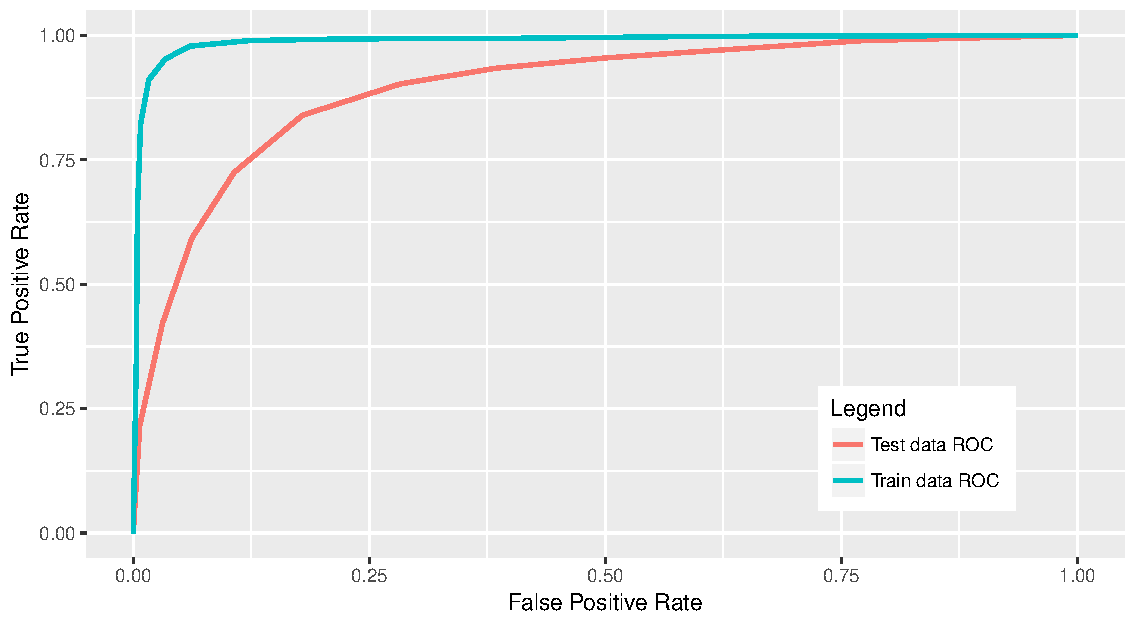
\includegraphics[width=8cm,height=7cm]{/LaTex/DiseaseNets/roc.PDF} % second figure itself
\centering \caption{The ROC curves for training data accuracy (blue) and for the test data (red). The overall accuracy on test data is 86\%}
\label{roc1}
\end{figure}
%%%%%%%%%%%%%%%%%%%%%%%%%%%%%%%%%%%%

The receiver operating characteristic curve (ROC) is based on evaluating the tradeoffs between specificity and sensitivity. Specificity is the probability of predicting a target given the true state is in fact a target, whereas sensitivity is the probability of predicting a non-target given the true state is a non-target. The classifier statistics are:\\

\noindent Accuracy = 86\% \\
Sensitivity = 0.87\\
Specificity = 0.84\\
Negative Predictive Value = 0.84\\
Positive Predictive Value = 0.87\\

The RandomForest classifier uses Gini index to rank each GO predictor term for it's contribution to discriminating between protein targets and non-targets. This information is displayed in table \ref{pred} with the highest scoring 15 predictors out of 149. 

%%%%%%%%%%%%%%%%%%%%%%%%%%%%%%%%%%%%
\begin{figure}[h]
\centering
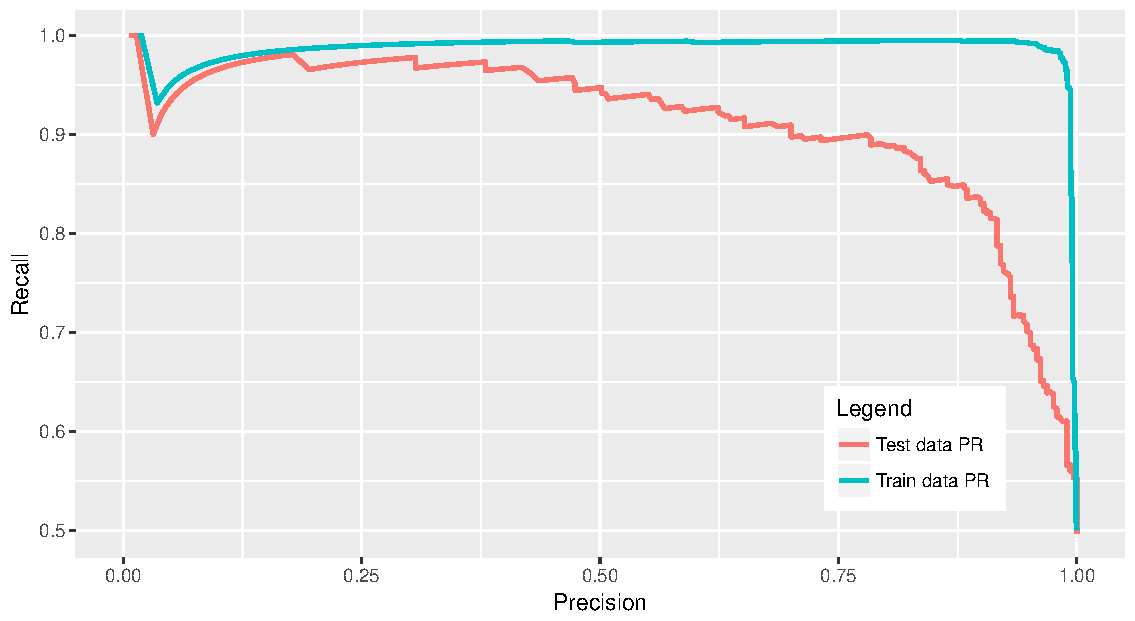
\includegraphics[width=8cm,height=7cm]{/LaTex/DiseaseNets/pr.PDF} % second figure itself
\centering \caption{The Precision and Recall curves for training data accuracy (blue) and for the test data (red).}
\label{pr1}
\end{figure}
%%%%%%%%%%%%%%%%%%%%%%%%%%%%%%%%%%%%

In figure \ref{pr1} the precision-recall curves are presented, this shows the precision values for corresponding sensitivity (recall) values. Similar to the ROC plot, the PR plot provides a model-wide evaluation. However, precision is directly influenced by class imbalance and does take the TN (true negatives) into consideration. The precision-recall curve highlights the tradeoff between precision and recall, where a high area under the curve represents both high recall and high precision, where high precision relates to a low false positive rate, and high recall relates to a low false negative rate. High scores for both criteria, indicate that the classifier is returning accurate results (high precision), as well as returning a majority of all positive results (high recall). Any classifier with high recall but low precision returns many results, but the majority of its predicted labels are incorrect when compared to the training labels. A classifier with high precision but with low recall will return very few results, but most of its predicted labels are correct when compared to the training labels. 

Examining figure \ref{pr1}, the blue line  indicates the train data and as such presents an almost perfect classifier. The test data indicated by the red curve presents a more realistic indication of the classifiers performance. Together with the ROC curve the precision-recall curve indicates the performance level for the  random forest.

% latex table generated in R 3.4.0 by xtable 1.8-2 package
% Sat Feb 10 08:53:21 2018
\begin{table}[ht]
\centering \scriptsize \caption{Top 15 GO Term predictor importance ranked on Gini score generated from the RandomForest classifier}
\label{pred}
\begin{tabular}{llll}
  \hline
 GOterm & Type &  Description & Value \\ 
  \hline
GO:0016301&MF&kinase activity & 86.37 \\ 
GO:0044281&BP&small molecule metabolic.process & 59.43 \\ 
GO:0043167&MF&ion binding & 30.58 \\ 
GO:0004871&MF&signal transducer activity & 29.86 \\ 
GO:0005886&CC&plasma membrane & 27.04 \\ 
GO:0055085&BP&transmembrane transport & 20.54 \\ 
GO:0022857&MF&transmembrane transporter activity & 20.17 \\ 
GO:0016491&MF&oxidoreductase activity & 18.89 \\ 
GO:0007165&BP&signal transduction & 14.61 \\ 
GO:0008233&MF&peptidase activity & 13.84 \\ 
GO:0006464&BP&cellular protein modification process & 12.03 \\ 
GO:0005615&CC&extracellular space & 11.58 \\ 
GO:0006950&BP&response to stress & 10.87 \\ 
GO:0042592&BP&homeostatic process & 9.04 \\ 
GO:0006810&BP&transport & 8.20 \\ 
   \hline \normalsize
\end{tabular}
\end{table}

The variable importance is calculated by the 'impurity' from the Gini index for splitting (deciding when to make splits on the input variables and when to stop growing the trees), at each split the importance of the variable is accumulated for every tree for that variable. For classification tasks such as this one, the Random Forest keeps a tally of each tree's output and then takes a majority vote to decide the overall class output. Further understanding of the classifier was gained when a breakdown of the GO terms giving frequency counts between targets and non-targets was made. 
%%%%%%%%%%%%%%%%%%%%%%%%%%%%%%%%%%%%
\begin{figure*}[h]
\centering
   \begin{subfigure}{0.5\linewidth} \centering
    \includegraphics[width=9cm,height=10cm]{/LaTex/DiseaseNets/nontarget-freqs.PDF}
     \caption{GO term frequencies for non-targets}\label{fig:fig1}
   \end{subfigure}
   \begin{subfigure}{0.4\linewidth} \centering
   \includegraphics[width=9cm,height=10cm]{/LaTex/DiseaseNets/target-freqs.PDF}
     \caption{GO term frequencies for targets}\label{fig:fig2}
   \end{subfigure}
\caption{The frequency counts for the presence (red bars) or absence (cyan) of a GO term for targets and non-targets. The y-axis is broken to highlight the differences between them. The {\it present'} category is generally the most predominant. The {\it absent} category is more frequent for the target proteins and thus discriminates between the non-targets} \label{fig:twofigs}
\end{figure*}
%%%%%%%%%%%%%%%%%%%%%%%%%%%%%%%%%%%%

The term GO:0016301 for kinase activity was the strongest variable with a score of 86.37,  the second key variable was term GO:0044281 for small molecule metabolic processes at 59.43. The third highest scoring variable was GO:0043167 which codes for ion binding with a value of 30.58. The majority of the 149 GO variables were scoring in single figures implying they were discriminating for small numbers of training samples.

Examining the frequency counts of the differences between the presence or absence of an ontological term is presented in figure \ref{fig:twofigs}. The frequency counts for the presence (red bars) or absence (cyan) of a GO term for targets and non-targets.  The {\it present'} category is generally the most predominant, the {\it absent} category is more frequent for the target proteins and thus discriminates between the non-targets. 

The k-core of a graph relates to the maximal connected subgraph, the vertices' of which must have at least of degree k within the subgraph. It is a useful technique for examining network connectivity where it is important to detect community and clusters. However, it can be quite interesting to visualize the coreness structure of small or medium networks, in figure \ref{coreness} were we show an example candidate protein and its neighbors. As a statistic, the numerical value of the k-coreness cannot identify potential targets, we examined the medians and IQR for the two groups and for targets the median=2, IQR=6, for nontargets median=5 and IQR=8.  The k-coreness is too over dispersed to discriminate between targets and nontargets but is useful for further analysis when targets are identified by the classifier.

%%%%%%%%%%%%%%%%%%%%%%%%%%%%%%%%%%%%
\begin{figure}[h]
\centering
  % \begin{subfigure}{0.3\linewidth} \centering
    \includegraphics[width=8.0cm,height=7cm]{/LaTex/DiseaseNets/APLP1.PDF}
     \caption{The protein APLP1 and its subnetwork indicating k-Coreness.The colors indicate the centrality of the subnetworks: red or yellow nodes are on the periphery, green and cyan represent the nearest neighbors while the central nodes are blue or purple. The plotting algorithm attempts to obtain a circular pattern where possible to highlight the k-cores}\label{coreness}
\end{figure}
%%%%%%%%%%%%%%%%%%%%%%%%%%%%%%%%%%%%

Examining the MIPS protein complex database it would appear that most  of the k-plex cores are part of protein complexes. We examined   the  most  significant  GO terms among k-plex core members are ranked and again we examined the protein types associated with these k-cores (between targets and non-targets).  The conclusion is that the location of a node is more important than the number of its connections or the number of connections of near neighbors. The coreness criteria is a better indicator of a node’s influence on biological function (target value) than degree.

The next stage of the analysis required generating a third list of proteins that were not drug targets  but had GoSlim ontology annotations. The first and second lists of proteins refer to the targets and non-targets used to build and test the RandomForest classifier. Third list proteins that were identified as target-like by the classifier were examined at the k-coreness level to determine network neighborhood and likely importance.

% Thu Jun 01 11:55:32 2017
\begin{table*}[h]
\centering \scriptsize \caption{Potential target proteins identified by RandomForest classifier and measures calculated for k-coreness criteria. Keeping proteins with probability ($>$0.7) and sorted by k-coreness ($>$ 1), we have 50 target protein candidates.}
\label{newtargets}
% latex table generated in R 3.4.0 by xtable 1.8-2 package
% Thu Apr 05 17:30:48 2018

\begin{tabular}{rllllr}
  \hline
 & TargetClass & Gene & myhubs & prob & core \\ 
  \hline
1 & Enzyme & PSMB9 & hub & 0.986 & 25.00 \\ 
  2 & Enzyme & ZDHHC17 & hub & 0.78 & 16.00 \\ 
  3 & Unknown & SQSTM1 & hub & 0.838 & 15.00 \\ 
  4 & Unknown & CRY1 & hub & 0.728 & 14.00 \\ 
  5 & Unknown & VPRBP & hub & 0.822 & 14.00 \\ 
  6 & Transporter & SLC39A8 & hub & 0.902 & 13.00 \\ 
  7 & Unknown & TNFSF8 & hub & 0.794 & 13.00 \\ 
  8 & Unknown & S100A8 & hub & 0.784 & 13.00 \\ 
  9 & Unknown & MRC2 & hub & 0.774 & 13.00 \\ 
  10 & Enzyme & DCT & hub & 0.85 & 13.00 \\ 
  11 & Enzyme & FBP1 & hub & 0.704 & 13.00 \\ 
  12 & Unknown & ITGAV & hub & 0.754 & 13.00 \\ 
  13 & Kinase & MAP3K8 & hub & 0.962 & 12.00 \\ 
  14 & Unknown & C8B & hub & 0.788 & 12.00 \\ 
  15 & Unknown & CD47 & hub & 0.898 & 12.00 \\ 
  16 & Unknown & NME2 & hub & 0.84 & 11.00 \\ 
  17 & TF & STAT5A & hub & 0.714 & 11.00 \\ 
  18 & IC & SCNN1D & hub & 0.826 & 10.00 \\ 
  19 & Enzyme & PAFAH1B1 & non-hub & 0.706 & 9.00 \\ 
  20 & Transporter & ABCG8 & hub & 0.946 & 9.00 \\ 
  21 & Unknown & AZGP1 & non-hub & 0.836 & 8.00 \\ 
  22 & Unknown & CFB & non-hub & 0.736 & 8.00 \\ 
  23 & IC & FXYD3 & non-hub & 0.788 & 8.00 \\ 
  24 & Kinase & NADK & non-hub & 0.834 & 7.00 \\ 
  25 & Enzyme & FUCA2 & non-hub & 0.766 & 7.00 \\ 
  26 & Enzyme & ARG1 & hub & 0.79 & 7.00 \\ 
  27 & Enzyme & ATP5A1 & non-hub & 0.762 & 7.00 \\ 
  28 & Kinase & SHPK & non-hub & 0.708 & 7.00 \\ 
  29 & Transporter & SLC20A2 & non-hub & 0.792 & 7.00 \\ 
  30 & Transporter & SLC39A10 & non-hub & 0.832 & 6.00 \\ 
  31 & Unknown & HPX & non-hub & 0.738 & 6.00 \\ 
  32 & Enzyme & CARD11 & non-hub & 0.766 & 5.00 \\ 
  33 & IC & ITPR1 & non-hub & 0.86 & 5.00 \\ 
  34 & Enzyme & ALDH1A3 & non-hub & 0.834 & 5.00 \\ 
  35 & Enzyme & F9 & hub & 0.736 & 5.00 \\ 
  36 & Unknown & VLDLR & non-hub & 0.82 & 4.00 \\ 
  37 & Enzyme & PEPD & non-hub & 0.706 & 4.00 \\ 
  38 & GPCR & OPN3 & non-hub & 0.726 & 4.00 \\ 
  39 & Kinase & ETNK2 & non-hub & 0.82 & 4.00 \\ 
  40 & Kinase & ITPK1 & non-hub & 0.738 & 4.00 \\ 
  41 & Enzyme & PPIP5K2 & non-hub & 0.762 & 4.00 \\ 
  42 & Transporter & SLC38A2 & non-hub & 0.74 & 4.00 \\ 
  43 & Unknown & PLEK & hub & 0.706 & 3.00 \\ 
  44 & GPCR & GPR22 & non-hub & 0.792 & 3.00 \\ 
  45 & Unknown & GJA5 & non-hub & 0.734 & 3.00 \\ 
  46 & Enzyme & GMPR & non-hub & 0.894 & 3.00 \\ 
  47 & Transporter & SLC2A6 & non-hub & 0.978 & 3.00 \\ 
  48 & Enzyme & SRD5A3 & non-hub & 0.77 & 2.00 \\ 
  49 & GPCR & FFAR2 & non-hub & 0.898 & 2.00 \\ 
  50 & Unknown & PRF1 & non-hub & 0.708 & 2.00 \\ 
    \hline
\end{tabular}
\end{table*}
\normalsize

In table \ref{newtargets} the list of potential protein targets identified by our system are displayed. They are ordered according to their probability score,  the likelihood they are target proteins. The first column gives the protein type, the second column identifies the protein name, the third column identifies the protein as a hub or non hub (based on our criteria),  the fourth column gives the probability score of the protein as a likely target (derived from the Random Forest outputs), the fifth column provides the k-coreness score, the final column informs of any evidence found from literature or other sources that the protein has been proposed as a drug target.

The final stage of the analysis takes the generated a list of candidate target proteins along with their characteristics as identified in table \ref{newtargets} and to place them them in the context of available drugs. Previous work by Yamanishi considered four possible approaches to this problem \cite{Yamanishi2008,Yamanishi2010}: (i) . new drug candidate compounds versus known target proteins, (ii) known drugs versus new target candidate proteins, (iii) new drug candidate compounds versus known target candidate proteins, (iv) known drugs versus known target candidate proteins. We  tackle class (ii), because we are introducing previously unknown/un-targeted  proteins.

Based on the protein class (e.g. enzyme, GPCR, Transporter etc) of our candidates we assessed the chemical structure and pharmacological properties of drugs targeting proteins of these types. We filled in missing protein class data from other sources. The characteristics of GPCR, Ion Channel, Transporter and enzyme class proteins were profiled based on the chemical structure and pharmacological similarity scores of the drugs targeting them.

Examining table \ref{newtargets} reveals that the highest scoring k-coreness proteins are generally hubs - that is to say they have over 17 connections to other proteins. However, the k-coreness score indicates they are centrally placed in the network. The majority of candidates are non-hubs with fewer connections although their k-coreness score is between 12 and 2. We examine the top scoring candidate target (PPIG) which is an enzyme and has been associated with diseases Bietti Crystalline Corneoretinal Dystrophy and Chronic Cystitis. It has a k-coreness rank of  15 and a neighborhood of 32 interconnected proteins, four of which have 13 drugs targeted at them. PPIG, therefore is located in a fairly active part of the drugome, a similarity search based on amino acid sequence reveals it is similar to  NKTR, PPID, and PPIL6.  None of these proteins have known drug targets, although PPID may be involved in anaplastic large cell lymphoma. Referring to table \ref{APLP1core} the drugs targeted at the three PPIG partners  are displayed.


% latex table generated in R 3.4.0 by xtable 1.8-2 package
% Sat Feb 17 10:46:11 2018
\begin{table}[h]
\centering \scriptsize \caption{The drug targeted proteins in the APLP1 module (k-coreness) network.}
\label{APLP1core}
\begin{tabular}{llll}
  \hline
 & DrugName & TargetClass & Gene \\ 
  \hline
2 & Mercaptopurine & Enzyme & PNP \\ 
  3 & Sorafenib & Unclassified & PNP \\ 
  4 & Brivudine & Kinase & TK1 \\ 
  5 & Idoxuridine & Kinase & TK1 \\ 
  6 & Zidovudine & Kinase & TK1 \\ 
  7 & Broxuridine & Kinase & TK1 \\ 
  8 & Sunitinib & Kinase & CDK4 \\ 
  9 & Quercetin & Kinase & CDK4 \\ 
  10 & Ruboxistaurin & Kinase & CDK4 \\ 
  11 & Ceritinib & Kinase & CDK4 \\ 
  12 & Nintedanib & Kinase & CDK4 \\ 
  13 & Ribociclib & Kinase & CDK4 \\ 
  14 & Pentamidine & Enzyme & SAT1 \\ 
   \hline \normalsize
\end{tabular}
\end{table}

The protein LGALS3 has been implicated in follicular adenoma of the thyroid gland, papillary carcinoma and malignant neoplasm of thyroid gland. Lactose is used to treat nodular goiter, supplement for loss of iodine. The CLK1 protein is involved in governing splice site selection. THAP1 is a nuclear proapoptotic factor that links prostate-apoptosis-response-4 nuclear bodies and has a number of associated diseases such as Dystonia 6, Torsion and Adolescent-Onset Dystonia Of Mixed Type. 

We accessed the STITCH database which contains experimental evidence and also predicted information, for the PPIG protein we may expect to find that Phenobarbital which is a long-acting barbiturate and the most widely used anti-seizure medication globally may interact with it. Also, arachidonic acid which is an essential fatty acid found in human fat as well as in the liver and brain may also interact with PPIG. The PPIG protein is centrally placed at the locus of several diseases, drugs and proteins thus may be playing an as yet unknown role. We examined the role of the top 10 proteins for evidence of potential use as drug targets, these are displayed in table \ref{evaluate}.

\begin{table}[h]
\centering \scriptsize \caption{Evaluation of the first 10 candidate target proteins. The larger the k-core, then usually more drugs will be involved in the network }
\label{evaluate}
\begin{tabular}{lllll}
  \hline
 Gene & k-core size & Drugs & Target & Evidence\\ 
  \hline
PSMA3  & 23 & 22 & Yes & (Tamura, 1991) \\ 
PPIG & 15 & 13 & No & (Nestell, 1996) \\ 
RPA2 & 15 & 30 & Yes & (Chaudhuri, 2004)\\ 
COL4A3BP & 17  &  9   & Yes & (Fugmann, 2007)\\
PTPRK & 13 & 53 & Yes & (Agarwal, 2013)\\ 
FXYD6 & 12 & 0 & No & (Xu, 2018)\\ 
FPR2 & 12 & 10 & Yes & (Klien, 1998)\\ 
SELE & 12 & 0 & No & None\\ 
KIR3DS1 & 12 & 1 & Tentative & (Carlomango, 2017)\\ 
%CHRNA9 & 41 & 12 & Yes & (Chikova, 2011)\\ 
ADAMTS2 & 12 & 1 & Tentative& (Wang,2017)\\ 
    \hline
\end{tabular}
\end{table}
\normalsize

The larger the k-core module the more likely there will be drugs already targeting the disease implicated proteins in the network neighborhood and this is confirmed information in table \ref{evaluate}. The PSMA3 (Proteasome subunit alpha type-3) protein  has two compounds for drug therapy, these also target the PSMA family of proteins. Furthermore, it is only recently that some of the protein candidates are becoming investigated as targets, such as the the KIR3DS1, FXYD6 and ADAMST2 proteins. In table \ref{evaluate} and also table \ref{newtargets}, it must be recalled that in the databases used in our study there is no mention of these proteins as targets. The Random Forest classifier has identified these proteins based on their gene ontology annotations. Some of the classifier discovered targets are in fact already targets, unfortunately this information was not available in our databases.  However, it has demonstrated the reliability and validity of our technique. 

\section{Conclusions}
The method described in this paper presents a novel approach for considering the viability of previously unrecognized/untargeted proteins as potential drug targets. We stress, that full validation can only be achieved through using in-vitro, animal tissue and ultimately, human tissue experiments. Our method provides an in-silico approach for generating lists of candidate targets that have rankings on several criteria such as biological similarities with known targets, protein type and complex network statistics describing the protein network neighborhood. The latter may play a role in the patient developing unwanted side-effects. We determined that both structure and connectivity patterns are necessary for identification of target proteins but this information needs to be coupled with biological knowledge. The use of Gene Ontology provides a biologically plausible method of protein annotation and assessment for further consideration as a target. In terms of limitations, we can say nothing about drug overall efficacy or long term effects on the predicted targets, the mode of drug action and pharmacological action is not considered. Future work will address the issues of drug repositioning in a principled way, using some of the methods described here.


\section*{Conflict of interests}
We declare that we have no conflicts of interest.

\section*{Acknowledgments}
We would like to thank the anonymous reviewers for their suggestions and comments which have improved the quality of the paper. We would also like to thank Kolaczyk and Csardi for developing the igraph package and Liaw for the RandomForest package.
\section*{References}  % elsart class does not automatically provide a section heading for references
\bibliographystyle{plainnat}
\bibliography{C:/Latex/kenrefs}
\end{document}



